% =====================================================================
\chapter{Metaheurísticas, optimización sin derivadas y multiobjetivo}
\label{tema:5}
% =====================================================================

Cuando el objetivo solo puede evaluarse (un simulador, un código heredado, un ensayo) o cuando la estructura del problema es tan irregular que ningún resolvedor exacto escala, se recurre a métodos que solo usan evaluaciones de $f$. Este tema sigue los capítulos~7 («Direct Methods»), 8 («Stochastic Methods»), 9 («Population Methods») y~12 («Multiobjective Optimization») de Kochenderfer y Wheeler~\cite{kw}, la clase~17 del curso 15.053~\cite{mit15053} para el recocido, y los artículos originales de Kirkpatrick, Gelatt y Vecchi~\cite{kirkpatrick} (recocido simulado), Hansen~\cite{hansen} (CMA-ES) y Deb \emph{et al.}~\cite{nsga2} (NSGA-II).

\section{Optimización de caja negra}

\begin{definicion}[Problema de caja negra]\label{def:caja-negra}
Un problema $\min_{x\in\mathcal{X}}f(x)$ es de \emph{caja negra} si solo se dispone de un oráculo que devuelve $f(x)$ (quizá con ruido) para cada $x$ consultado, sin gradientes ni estructura explícita. Su coste se mide por el \emph{número de evaluaciones}.
\end{definicion}

Hay dos regímenes. Si cada evaluación es barata (milisegundos), se pueden permitir miles o millones de evaluaciones y se usan metaheurísticas. Si es cara (horas de simulación o un experimento de planta), cada evaluación debe elegirse con cuidado con un modelo sustituto, como en la optimización bayesiana~\cite{garnett,frazier}, que la fase desarrolla más adelante. Los métodos directos locales, como Nelder--Mead o Powell (cap.~7 de~\cite{kw}), son adecuados cuando el problema es continuo, de pocas variables y con un único valle.

\section{Recocido simulado}

El recocido simulado~\cite{kirkpatrick} imita el enfriamiento lento de un metal. Desde una solución $x$ se propone un vecino $x'$ (por ejemplo, intercambiar dos departamentos) con un mecanismo simétrico, $\Prob(x\to x')=\Prob(x'\to x)$, y se acepta con la probabilidad de Metropolis
\[
\alpha(x,x')=\min\Bigl(1,\ e^{-(f(x')-f(x))/T}\Bigr),
\]
donde la temperatura $T>0$ disminuye según un calendario, típicamente $T_{k+1}=\rho T_k$ con $\rho\in(0{,}9;\ 0{,}999)$. Con $T$ alta se aceptan muchos empeoramientos y se explora; con $T$ baja solo se aceptan mejoras y se explota.

\begin{proposicion}[Distribución estacionaria de Boltzmann]\label{prop:boltzmann}
Sea $\mathcal{X}$ finito, la propuesta simétrica e irreducible y $T$ fija. La cadena de Markov del recocido satisface el equilibrio detallado con
\[
\pi_T(x)=\frac{e^{-f(x)/T}}{\sum_{z\in\mathcal{X}}e^{-f(z)/T}},
\]
que es por tanto una distribución estacionaria. Cuando $T\to 0$, $\pi_T$ se concentra uniformemente en el conjunto de mínimos globales.
\end{proposicion}

\begin{proof}
Para $x\ne x'$, la probabilidad de transición es $P(x,x')=\Prob(x\to x')\,\alpha(x,x')$. Supóngase $f(x')\ge f(x)$. Entonces $\alpha(x,x')=e^{-(f(x')-f(x))/T}$ y $\alpha(x',x)=1$, y
\[
\pi_T(x)P(x,x')\propto e^{-f(x)/T}\,\Prob(x\to x')\,e^{-(f(x')-f(x))/T}=e^{-f(x')/T}\,\Prob(x'\to x)\propto\pi_T(x')P(x',x).
\]
El caso $f(x')<f(x)$ es simétrico. Sumando el equilibrio detallado sobre $x$ se obtiene $\sum_x\pi_T(x)P(x,x')=\pi_T(x')$. Para el límite, sea $f^{*}=\min f$ y $\mathcal{X}^{*}$ el conjunto de minimizadores: $\pi_T(x)=e^{-(f(x)-f^{*})/T}/\sum_z e^{-(f(z)-f^{*})/T}$; el numerador tiende a~1 si $x\in\mathcal{X}^{*}$ y a~0 en otro caso, y el denominador tiende a $\abs{\mathcal{X}^{*}}$.
\end{proof}

La distribución de Boltzmann es la del módulo~6 (tema~5). La garantía de convergencia al óptimo exige calendarios logarítmicos, demasiado lentos; en la práctica se usa el geométrico y varias ejecuciones independientes.

\section{Algoritmos genéticos y estrategias evolutivas}

Un \emph{algoritmo genético} mantiene una población de soluciones y la renueva con tres operadores (cap.~9 de~\cite{kw}): \emph{selección} de padres favoreciendo a los mejores (por ejemplo, por torneo entre dos individuos al azar), \emph{cruce} que combina dos padres y \emph{mutación} que perturba un hijo. Con \emph{elitismo} los mejores pasan intactos a la generación siguiente. La representación debe respetar las restricciones: para permutaciones, el \emph{cruce por orden} (OX) copia un tramo del primer padre y completa los huecos con los genes que faltan en el orden en que aparecen en el segundo, de modo que el hijo sigue siendo una permutación.

\begin{definicion}[CMA-ES]\label{def:cmaes}
La \emph{estrategia evolutiva con adaptación de la matriz de covarianza} (CMA-ES)~\cite{hansen} optimiza en $\R^{n}$ manteniendo una distribución $\mathcal N(m,\sigma^{2}C)$. En cada generación:
\begin{enumerate}[label=\arabic*.]
  \item muestrea $\lambda$ candidatos $x_k=m+\sigma y_k$, con $y_k\sim\mathcal N(0,C)$, y los ordena por $f$;
  \item actualiza la media con los $\mu$ mejores: $m\leftarrow\sum_{i=1}^{\mu}w_ix_{i:\lambda}$, con pesos positivos decrecientes que suman~1; la referencia propone $w_i\propto\ln\frac{\lambda+1}{2}-\ln i$;
  \item actualiza $C$ con los pasos que tuvieron éxito (actualizaciones de rango uno y de rango $\mu$) y ajusta $\sigma$ comparando la longitud del camino evolutivo con la esperada bajo selección aleatoria.
\end{enumerate}
El \emph{tamaño efectivo de selección} es $\mu_{\mathrm{eff}}=1/\sum_iw_i^{2}$.
\end{definicion}

CMA-ES aprende la forma del valle: en un problema mal condicionado, $C$ tiende a una matriz proporcional a la inversa del hessiano, de modo que se comporta como un método de segundo orden sin derivadas. Es invariante a transformaciones monótonas de $f$ (solo usa el orden) y a rotaciones del espacio. Es una elección sólida para calibrar simuladores de caja negra con decenas de parámetros continuos y miles de evaluaciones posibles.

\section{Optimización multiobjetivo}

\begin{definicion}[Dominancia y frente de Pareto]\label{def:pareto}
Sea $F=(f_1,\dots,f_k)$ un vector de objetivos que se minimizan. Se dice que $x$ \emph{domina} a $x'$, $x\succ x'$, si $f_i(x)\le f_i(x')$ para todo $i$ y $f_j(x)<f_j(x')$ para algún $j$. Un punto factible es \emph{Pareto-óptimo} si ningún otro punto factible lo domina. La imagen $F(\mathcal{X}^{\mathrm{P}})$ del conjunto de Pareto-óptimos es el \emph{frente de Pareto}.
\end{definicion}

\begin{proposicion}[Suma ponderada]\label{prop:suma-ponderada}
Si $w_i>0$ para todo $i$ y $x^{*}$ minimiza $\sum_iw_if_i(x)$ en $\mathcal{X}$, entonces $x^{*}$ es Pareto-óptimo. El recíproco es falso: los puntos del frente que no están en la frontera de su envolvente convexa no minimizan ninguna suma ponderada.
\end{proposicion}

\begin{proof}
Si algún $x$ dominase a $x^{*}$, sería $f_i(x)\le f_i(x^{*})$ para todo $i$, con desigualdad estricta en algún $j$; como todos los pesos son positivos, $\sum_iw_if_i(x)<\sum_iw_if_i(x^{*})$, en contra de la minimalidad. Para el recíproco, el \cref{ej:planta} da un contraejemplo.
\end{proof}

El método de la $\varepsilon$-restricción, $\min f_1$ s.a. $f_2\le\varepsilon$, sí alcanza los puntos no apoyados variando $\varepsilon$ (\cref{eje:5-eps}). Para problemas de caja negra, el \emph{NSGA-II}~\cite{nsga2} combina un algoritmo genético con dos ideas:
\begin{enumerate}[label=(\alph*)]
  \item \emph{ordenación no dominada}: la población se divide en frentes $\mathcal{F}_1$ (no dominados), $\mathcal{F}_2$ (no dominados al quitar $\mathcal{F}_1$), etc., y el rango de un individuo es el índice de su frente;
  \item \emph{distancia de aglomeración} (\emph{crowding distance}): dentro de un frente, para cada objetivo se ordenan los puntos, los extremos reciben distancia infinita y cada punto interior suma $(f_k^{\text{sig}}-f_k^{\text{ant}})/(f_k^{\max}-f_k^{\min})$; se prefieren los puntos aislados para mantener la diversidad.
\end{enumerate}
La selección por torneo compara primero el rango y después la distancia, y la nueva generación se forma con los mejores frentes de la unión de padres e hijos (elitismo).

\begin{ejemplo}[Caso de estudio: distribución en planta]\label{ej:planta}
Una nave industrial tiene seis módulos en una cuadrícula de $2\times 3$ con centros separados 20~m; las carretillas circulan por pasillos ortogonales, de modo que la distancia entre módulos es la de Manhattan. Hay que asignar seis departamentos: Recepción (R), Almacén (A), Mecanizado (M), Soldadura (S), Pintura (P) y Expedición (E). Los viajes diarios de carretilla entre departamentos son R--A: 30, A--M: 25, A--S: 10, A--E: 5, M--S: 20, M--P: 5, S--P: 25 y P--E: 30.

\emph{Objetivos.} (1) Recorrido de carretillas $f_1(\pi)=\sum_{i<j}F_{ij}\,d_{\pi(i)\pi(j)}$ (m/día), con $\pi(i)$ el módulo del departamento $i$. (2) Riesgo por proximidad de departamentos incompatibles, $f_2(\pi)=\sum w_{ij}\cdot 20/d_{\pi(i)\pi(j)}$, con pesos 10 para soldadura--pintura (chispas y disolventes), 4 para mecanizado--pintura (polvo) y 3 para soldadura--almacén; vale $w_{ij}$ si los dos departamentos son contiguos y disminuye con la distancia.

\emph{Elección del método.} Es un problema cuadrático de asignación, NP-difícil en general. Con seis departamentos hay $6!=720$ distribuciones, lo que permite certificar por enumeración lo que hacen las metaheurísticas; con 30 departamentos ($\approx 2{,}7\cdot 10^{32}$) solo quedarían estas.

\emph{Resultados} (cuaderno, parte~5).
\begin{enumerate}[label=(\alph*)]
  \item El recorrido mínimo es \textbf{3400~m/día}, alcanzado por 16 distribuciones (simetrías de la cuadrícula). El recocido con intercambios, $T_0=500$, $\rho=0{,}995$ y 3000 iteraciones lo encuentra en las cinco semillas probadas.
  \item El frente de Pareto tiene cuatro puntos: $(3400;\ 13{,}5)$, $(3700;\ 10{,}5)$, $(3900;\ 7{,}83)$ y $(4400;\ 6{,}83)$. El punto $(3700;\ 10{,}5)$ no lo alcanza ninguna suma ponderada: el segmento que une $(3400;\ 13{,}5)$ y $(3900;\ 7{,}83)$ pasa en $f_1=3700$ por $f_2=13{,}5-0{,}6\cdot 5{,}67=10{,}1<10{,}5$, de modo que el punto queda por encima de la envolvente convexa.
  \item Un NSGA-II mínimo (población 40, 40 generaciones, cruce OX y mutación por intercambio) recupera los cuatro puntos del frente en 0,3~s.
\end{enumerate}
La \cref{fig:planta} muestra dos distribuciones del frente. Con $f_1$ mínimo, el flujo sigue una U (R--A--M abajo, S--P--E arriba), pero soldadura y pintura quedan contiguas. Separándolas cuesta 500~m/día más de carretilla y el riesgo baja de 13,5 a 7,83. Elegir entre ellas no es tarea del algoritmo, sino de quien conoce el valor relativo del riesgo y del tiempo de transporte.
\end{ejemplo}

\begin{figure}[h]
\centering
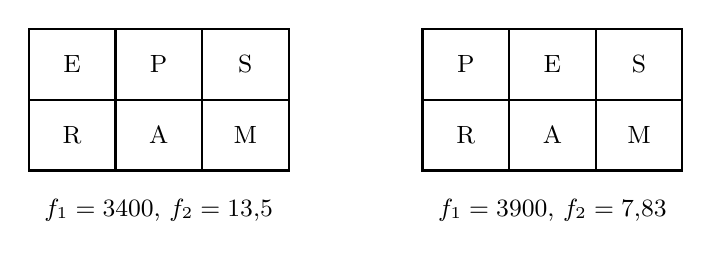
\begin{tikzpicture}[font=\small,cel/.style={draw,thick,minimum width=11mm,minimum height=9mm}]
  \begin{scope}
    \foreach \t [count=\i from 0] in {R,A,M} \node[cel] at (1.1*\i,0) {\t};
    \foreach \t [count=\i from 0] in {E,P,S} \node[cel] at (1.1*\i,0.9) {\t};
    \node[align=center] at (1.1,-0.95) {$f_1=3400$, $f_2=13{,}5$};
  \end{scope}
  \begin{scope}[xshift=5cm]
    \foreach \t [count=\i from 0] in {R,A,M} \node[cel] at (1.1*\i,0) {\t};
    \foreach \t [count=\i from 0] in {P,E,S} \node[cel] at (1.1*\i,0.9) {\t};
    \node[align=center] at (1.1,-0.95) {$f_1=3900$, $f_2=7{,}83$};
  \end{scope}
\end{tikzpicture}
\caption{Dos distribuciones Pareto-óptimas del caso de la planta. A la izquierda, mínimo recorrido; a la derecha, soldadura y pintura separadas por expedición.}
\label{fig:planta}
\end{figure}

\begin{table}[h]
\centering\small
\caption{Tecnologías del tema~5: metaheurísticas y multiobjetivo.}\label{tab:tec5}
\begin{tabularx}{\textwidth}{@{}l>{\raggedright\arraybackslash}X>{\raggedright\arraybackslash}p{2.2cm}>{\raggedright\arraybackslash}X@{}}
\toprule
Herramienta & Para qué sirve & Licencia o tipo & Cuándo elegirla \\
\midrule
\texttt{cma} (Hansen \emph{et al.}) & CMA-ES de referencia, con restricciones de caja y ruido & abierta (BSD-3) & calibrar simuladores continuos de caja negra \\
pymoo~\cite{pymoo} & NSGA-II, NSGA-III, indicadores de calidad de frentes & abierta (Apache~2.0) & problemas multiobjetivo con operadores estándar \\
SciPy \texttt{optimize} & recocido dual, evolución diferencial, Nelder--Mead, Powell & abierta (BSD-3) & continuo, pocas variables, sin dependencias extra \\
Optuna & búsqueda de hiperparámetros (muestreadores TPE y CMA-ES, multiobjetivo) & abierta (MIT) & ajustar modelos o configuraciones con evaluaciones caras \\
Código propio & recocido, búsqueda tabú, genéticos sobre una representación específica & propio & combinatoria con vecindarios propios del dominio \\
\bottomrule
\end{tabularx}
\end{table}

\begin{observacion}[Errores frecuentes con metaheurísticas]\label{obs:errores5}
\begin{enumerate}[label=(\alph*)]
  \item \emph{Conclusiones con una sola semilla}: un resultado estocástico se informa con varias ejecuciones (media, peor caso, dispersión) y con el mismo número de evaluaciones para todos los métodos comparados.
  \item \emph{Ajustar hiperparámetros sobre la instancia de evaluación}: igual que en aprendizaje automático, es sobreajuste; se ajustan en instancias de entrenamiento y se evalúan en otras.
  \item \emph{Restricciones como penalizaciones mal escaladas}: con penalización pequeña la solución final es infactible; con una enorme el paisaje se vuelve plano. Mejor representaciones que garanticen la factibilidad o una reparación explícita.
  \item \emph{Ruido en la evaluación}: con un simulador estocástico, el mejor valor observado está sesgado a la baja (maldición del optimizador, \cref{tema:6}); hay que reevaluar el candidato final con nuevas réplicas.
  \item \emph{Presentar el frente sin decidir}: un frente con cien puntos no es una decisión; hay que acordar con el usuario las preferencias o el punto de compromiso.
\end{enumerate}
\end{observacion}

\begin{lecturas}
\item Kochenderfer y Wheeler~\cite{kw}, caps.~7 «Direct Methods», 8 «Stochastic Methods», 9 «Population Methods» y~12 «Multiobjective Optimization».
\item S.~Kirkpatrick, C.~D. Gelatt y M.~P. Vecchi~\cite{kirkpatrick}, artículo original del recocido simulado.
\item N.~Hansen~\cite{hansen}, tutorial de CMA-ES.
\item K.~Deb \emph{et al.}~\cite{nsga2}, artículo original de NSGA-II.
\end{lecturas}

\section*{Ejercicios del tema 5}
\addcontentsline{toc}{section}{Ejercicios del tema 5}

\begin{ejercicio}{1}{eje:5-aceptacion}
Un movimiento empeora el objetivo en $\Delta=50$. Calcule su probabilidad de aceptación con $T=100$ y con $T=25$. Con el calendario $T_{k+1}=0{,}99\,T_k$ y $T_0=500$, ¿cuántas iteraciones hacen falta para que $T<1$?
\fuente{adaptado de MIT 15.053, primavera de 2013, clase~17, recocido simulado con enfriamiento $T:=0{,}99\,T$~\cite{mit15053}.}
\end{ejercicio}

\begin{ejercicio}{2}{eje:5-frentes}
Seis soluciones de un problema con dos objetivos que se minimizan tienen imágenes $a=(1,9)$, $b=(2,7)$, $c=(3,8)$, $d=(4,4)$, $e=(5,5)$ y $f=(7,2)$. Calcule los frentes de la ordenación no dominada y el rango de cada solución.
\fuente{adaptado de K.~Deb \emph{et al.}~\cite{nsga2}, ordenación rápida no dominada.}
\end{ejercicio}

\begin{ejercicio}{2}{eje:5-crowding}
Calcule la distancia de aglomeración de los puntos del primer frente del \cref{eje:5-frentes}. ¿Cuál se descartaría primero si hubiera que eliminar uno que no sea extremo?
\fuente{adaptado de K.~Deb \emph{et al.}~\cite{nsga2}, distancia de aglomeración.}
\end{ejercicio}

\begin{ejercicio}{2}{eje:5-apoyado}
Con los cuatro puntos del frente del \cref{ej:planta}, demuestre que no existe ningún peso $w\in[0,1]$ tal que $(3700;\ 10{,}5)$ minimice $wf_1+(1-w)f_2$ entre ellos.
\end{ejercicio}

\begin{ejercicio}{2}{eje:5-ox}
Aplique el cruce por orden (OX) a los padres $p_1=(1,2,3,4,5,6)$ y $p_2=(4,6,2,1,5,3)$ copiando de $p_1$ las posiciones 3 a~5 y rellenando el resto de izquierda a derecha con los genes que faltan en el orden en que aparecen en $p_2$. Compruebe que el hijo es una permutación.
\end{ejercicio}

\begin{ejercicio}{2}{eje:5-pesos}
Para CMA-ES con $\lambda=6$ candidatos y $\mu=3$ padres, calcule los pesos $w_i\propto\ln\frac{\lambda+1}{2}-\ln i$, normalizados para sumar~1, y el tamaño efectivo $\mu_{\mathrm{eff}}$.
\fuente{adaptado de N.~Hansen~\cite{hansen}, elección por defecto de los pesos de recombinación.}
\end{ejercicio}

\begin{ejercicio}{3}{eje:5-eps}
(a) Demuestre que toda solución óptima única de $\min f_1(x)$ s.a. $f_2(x)\le\varepsilon$ es Pareto-óptima. (b) Muestre con el \cref{ej:planta} que eligiendo $\varepsilon$ adecuadamente se obtiene el punto $(3700;\ 10{,}5)$, que la suma ponderada no alcanza.
\fuente{adaptado de Kochenderfer y Wheeler~\cite{kw}, cap.~12, métodos de restricción para el frente de Pareto.}
\end{ejercicio}

\begin{ejercicio}{3}{eje:5-metropolis}
Demuestre que si la propuesta del recocido no es simétrica, la aceptación de Metropolis--Hastings $\alpha(x,x')=\min\bigl(1,\ e^{-(f(x')-f(x))/T}\,\Prob(x'\to x)/\Prob(x\to x')\bigr)$ restaura el equilibrio detallado con $\pi_T$. Explique por qué un error en esa corrección sesga la búsqueda hacia las regiones donde la propuesta concentra su masa.
\fuente{adaptado de Kochenderfer y Wheeler~\cite{kw}, cap.~8, y de S.~Kirkpatrick \emph{et al.}~\cite{kirkpatrick}.}
\end{ejercicio}
